\documentclass[oneside, 12pt]{extbook}

% imports + page geometry
\usepackage{geometry}
\usepackage{graphicx}
\usepackage{listings}
%\usepackage{physics}
\usepackage[dvipsnames]{xcolor}
\usepackage[italian]{babel}
\usepackage{amsmath}
\usepackage{mathtools}

\DeclarePairedDelimiter{\abs}{\lvert}{\rvert}

\geometry{
        a4paper, 
        top = 2cm,
        left = 1.5cm,
        right = 1.5cm,
        bottom=2cm
}

\title{Hardware, Electromagnetic and Localization Security}
\author{Pierciro Caliandro}



\begin{document}
\maketitle
\chapter{Introduzione}
\section{Introduzione}
Attacco fisico invece di informatico, viene applicato un attacco di tipo EM: si mandano segnali fisici su un apparato per indurre malfunzionamento o rubare dati.\\Si arriva all'impatto sull'elettronica, si cerca quindi di ottenere dei rudimenti di sicurezza fisica: 3 aspetti di livello diverso, dal sistema, alla parte di comunicazione alla parte elettronica.\\Aspetti fondamentali:\\
- short range vulnerabilities: dispositivi medici avranno tutte funzionalità wireless: pacemakers va configurato, quindi in base alla risposta configura il dispositivo con un accoppiamento di tipo NFC, in futuro anche le protesi più "sciocche" come una placca per le ossa saranno wireless, sarà funzionalizzato con diversi sensori per verificare infezioni etc... ed essere letto da fuori.\\Qualunque oggetto impiantato sarà funzionalizzato, a seguito di interventi di qualunque tipo (punti di sutura etc...) che sarà provvisto di sensori.\\È tutto vittima di attacco informatico, per rubare dati in maniera non intenzionale.\\Il corpo diventa quindi un nodo di Internet, si parla di \textbf{Internet of the bodies}, ci possono essere diversi tipi di sensori che interagiscono.C'è una lista svariata di oggetti di medica che controllano le attività fisiche.\\L'accesso non intenzionale al dispositivo ha un impatto potenzilamente dirompente, lo scenario va a parare in una medicina guidata dai dati dove si mischiano diverse discipline, è il concetto di \textbf{medicina di precisione}: parte dalle terapie oncologiche, in ingegneria è la capacità della medicina di apprendere. Se la terapia oggi va bene, il corpo umano cambia e quindi tale terapia può necessitare di essere aggiornata.\\Il punto critico è che per rendere questa visione operabile, occorre avere sistemi pervasivi + AI per poter poi tirare fuori una cura.\\È una medicina assistiva che può essere integrata con sensori nella casa che controllano l'utente paziente, si parla di 3 tipi di dispositivi, ci interessa capire come questi comunicano e non il loro funzionamento:
\begin{itemize}
    \item wearable
    \item epidermici
    \item implantable
\end{itemize}
che devono avere la safety by design, quindi non devono fare male quando indossati, la security by design e quindi essere sicuri da progettazione e poi la privacy by design, quindi capire come è possibile che i dati vengano usati impropriamente.\\Abbiamo ad esempio strumenti epidermici che rilascia cortisolo quando ad esempio viene misurato da un sensore che scende sotto soglia una certa misura.\\Ci sono quindi 3 tipi di links:
\begin{itemize}
    \item on-body link
    \item through-the-body
    \item off-the-body
\end{itemize}
Analizzeremo tutto a livello di modello fisico-matematico.\\Ci sono poi problemi per quanto riguarda la lettura dei dati, qui c'è la corrispondenza fisica di come si leggono tali dati, ma c'è anche il come si fa per accedere al dispositivo, ad esempio ci sono delle micro-antenne non volute.
\subsection{Introduzione generale sulla cybersecurity}
Si completa il concetto di cybersecurity con gli aspetti fisici e di comunicazione, vi sono delle criticità nelle comunicazioni sulla rete. Ce ne sono però alcune che non vengono prese in considerazione spesso, che è opportuno non tralasciare come appunto la comunicazione a corto raggio: si viaggia in ambienti affollati per rubare dati da cellulari ad esempio se è abilitato il sistema NFC. Normalmente la distanza è dell'ordine del metro, ma su un posto affollato è fattibile, il lettore viene posto vicino al cellulare e ruba dati.\\Per le reti ad ampio raggio, ci sarà la sicurezza delle reti da cui però rimangono fuori tutta una serie di apparati che sono ad esempio i sistemi di localizzazione. Ormai quasi tutte le applicazioni usano la posizione per fare delle operazioni, usano EMF per portare dati e sono attaccabili: è "facile" far credere ad un device di trovarsi in un luogo anzi che in un altro.\\È stato dimostrato che era possibile controllare uno yatch di lusso semplicemente ingannando il sistema di navigazione, ad esempio.È ancora più semplice inibire i servizi, quindi fare in modo che il servizio non funzioni e basta, un'altra applicazione è quella di sfruttare le EMF usate nei radar per capire dove si trova qualche oggetto, quindi disturbare un radar vuol dire interrompere il funzionamento di un sistema target a bassi rischi.\\Cerchiamo quindi di capire come disturbare o difendere un sistema di navigazione o un radar, per cercare di capire come proteggerli nel mondo reale.\\Entreremo poi nell'hardware, vedendo vari metodi su come attaccare l'hardware stesso: anche qui, si da per acquisito che il chip sia sicuro in quanto non si può aprire ed occorre per forza passare per il software, ma in realtà negli anni vi sono stati una serie di side channel, come ad esempio isolare termicamente un device.\\Ma se si può monitorare la temperatura del device, è possibile capire che elaborazioni sta facendo e quindi capire le attività dell'utente, questo vale anche per le RAM etc... ad esempio vedere quanto sono frequenti le rotture delle singole celle della RAM etc...\\
\subsection{Sicurezza informatica e cybersecurity}
È un concetto molto ampio, spesso confuso con la cybersecurity, ma la prima vuol dire mantenere in sicurezza l'informazione anche se non è digitale. Non basta quindi proteggersi da attacchi via rete, il concetto è molto più ampio della cybersceurity. Ci sono tantissime definizioni standard per cybersecurity, ma è meglio partire da un approccio che vede il sistema moderno come formato da tante entità, che possiamo dividere in 3 parti:
\begin{itemize}
    \item hardware, che non è per forza l'hardware del calcolatore, anche un banale pezzo di carta con su scritta una password.
    \item software, l'hardware visto da un punto di vista informatico è correlato con programmi applicativi che possono avere delle debolezze, occorre quindi anche proteggere l'interno della macchina
    \item parte di comunicazione, in quanto il mondo moderno di IoT o cloud prevede che l'informazione viaggi fra utente e server o fra vari utenti
\end{itemize}
La maggior parte delle informazioni continuano a mandare informazioni a qualche server chissà dove (magari in CINA \textbf{cit}), in questo modo ci sono diverse facilitazioni.\\\\Questo vuol dire aver venduto parte della privacy a qualcuno o comunque delegato, che non è detto che sia malvagio ma c'è una comunicazione che avviene continuamente e quindi potrebbe interessare a qualcun altro per intervenire sul canale di comunicazione ed entrare in casa.\\Questo rimanendo ancora nell'accezione più classica della comunicazione, ma abbiamo anche comunicazione a livello di corto raggio, quindi per gestire queste 3 componenti principali occorre mettere in atto tutta una serie di contromisure che non sono solo quelle che vederemo ma sono molto più ampie:\\
- procedure di autenticazione, come il controllo di accessi in un edificio, ci possono essere informazioni che vengono classificate come sensibili ed a cui non si può accedere (es. badge per accedere a determinati uffici). Già questo aspetto se ben fatto sarebbe una grossa protezione, soprattutto per software ed hardware security in quanto vorrebbe dire avere degli alti livelli di sicurezza
- sicurezza a livelli più bassi, CIA: Confidentiality, Availability and Integrity. Devono valere questi 3 principi nell'information security:
- C è un concetto diverso dalla privacy, sta proprio nel non rivelare l'informazione che non dovrebbe essere nota.
- I, ovvero la capacità del sistema di non perdere le informazioni che può essere accidentale o anche dovuta ad attacchi, esempi come i ransomware possono portare ad avere dei costi. Ci sono anche altre tipi di compromissione di integrità, che riguardano ad esempio il disturbo di un segnale riguardo la posizione
- A, il fatto che l'informazione sia integra non vuol dire che possa essere utilizzata.Ad esempio se si perde la password per accedere a determinati dati, mantenerle ha un suo costo\\\\Vedremo come declinare queste 3 caratteristiche nei casi di studio del corso.\\\\Ci sono delle definizioni da dare:
\begin{itemize}
    \item vulnerabilità: sfruttate dall'attaccantte, qualsiasi sistema ha una debolezza da qualche parte nella sua progettazione. Se può essere sfruttata per ridurre una delle 3 cose, possiamo chiamare tale debolezza una vulneraiblità
    \item un cyber attacco sfrutta la vulnerabilità per ridurre la sicurezza.\\\\Più comuni tecniche di attacco:\\
    \item backdoor: vie lasciate aperte dagli sviluppatori, come porte aperte etc... 
    \item DoS: negazione del servizio, si fa in modo che per qualche motivo il servizio sotto attacco divenga indisponibile, come ad esempio richieste di accesso ad un server molteplici volte. Nella parte wireless è molto usato, mediante il \textbf{jammer}: è un sistema che trasmette con la massima potenza possibile sul canale usato dal sistema per comunicare, che disturba la comunicazione fino a negare il canale per comunicare. È una tecnologia banale per effettuare DoS 
    \item attacchi ad accesso diretto non autorizzato.
    \item eavesedropping, dove si ascolta e se ci sono delle informazioni riservate si possono captare.\\Esempio: canale della DSB, ogni aereo mette la posizione, è un canale in chiaro e quindi ascoltare ed usare quei dati in modo malevolo può creare problemi. 
    \item phishing
    \item privilege escalation
    \item social engineering
    \item reverse engineering
    \item side channel attack: verificare dei canali correlate con l'informazione da difendere o attaccare, per capire cosa sta succedendo. 
    \item spoofing: attacco che tende a confondere la persona o entità sotto attacco mediante l'invio di falsi dati. Si presta bene alla comunicazione wireless, molto usato nei sistemi di localizzaizone tipo GPS peché è noto a tutti come è standardizato il segnale che arriva al satellite e quindi si può ricostruire e trasmettere. Ma quando lo si ricostruisce si inseriscono delle false informazioni, per far ad esempio cambiare posizione al GPS.
    \item tampering: alterazione fisica del dispositivo
    \item malware
\end{itemize}
È importante inoltre ribadire la differenza fra sicurezza intesa come
- safety: concetto che esprime la capacità di mettersi ala riparo da accadimenti dannosi per l'uomo e per la vita umana. Ad esempio la precipitazione dell'aereo, mantenere tale proprietà occorre salvaguardarsi da qualsiasi cosa può accadere. Ad esempio, un aereo può precipitare perché il sistema di comunicazione si danneggia o interferisce con un altro 
- security: la security è correlata, ma non è sovrapposta bensì è come "un ombrello" che permette di mantenere la safety.\\Se installiamo un sistema di sicurezza in casa, veniamo protetti da chi vuole entrare, ma non dal fatto di poter cadere e battere la testa scivolando nella vasca (\textbf{super cit}.\\\\Ci occuperemo della security, ma molte delle cose che vederemo possono o non possono essere usate anche per garantire la safety.\\È inoltre importante tenere a mente che ormai l'ambiente è pieno di EMF, quindi lo spettro EM è molto pieno e quindi aggiungere qualche altra fonte diventa semplice, quindi vedremo questa cosa.

\part{Parte Electromagnetic}
\chapter{Lezione 2}
\section{Interazione elettromagnetica col corpo umano}
Cosa accade quando una onda EM interagisce col corpo umano: occorre sapere cosa succede perché quando un dispositivo deve essere immesso nel mercato deve garantire la safety: vincolo sulla potenza che rilascia nel corpo umano. È un vincolo di progetto, occorre capire cosa si intende per potenza che entra nel corpo umano, occorre anche sapere che succede quando un dispositivo riceve un'onda EM per non far funzionare il dispositivo.\\Quando un onda investe il corpo umano, abbiamo un'onda elettrica ed una magnetica che investono il corpo umano e quindi 3 fenomeni:
\begin{itemize}
    \item propagazione
    \item riscaldamento, dovuto all'assorbimento di potenza
    \item effetti chimico-fisici
\end{itemize}
Ci interessa come punto fondamentale la propagazione, il riscaldamento è un effetto. In altri contesti, l'obiettivo è scaldare il corpo (come nella fisioterapia), ma comunque occorre capire anche cosa accade perché l'assorbimento di potenza produce dei vincoli che occorre tenere conto.\\Questi fenomeni sono legati a:
\begin{itemize}
	\item materiale
	\item frequenza: cambierà in base a che tipo di oggetto sta irradiando, come sono fatti i tessuti etc...
\end{itemize}
Tipicamente,l'esposizione del campo sul corpo produce delle correnti, quando consideriamo l'interazione col corpo umano abbiamo 4 tipi di correnti:
\begin{itemize}
	\item correnti di conduzione: sono legate alla presenza di elettroni liberi, ad esempio se ci sono dei fluidi.\\ Gli elettroni, quando si applica un campo E, tenderanno a muoversi in una determinata direzione secondo la \textbf{legge di Ohm}:
	\begin{equation}
		\underline{J} = \sigma \cdot \underline{E}
	\end{equation}
	\item correnti di convezione: dovuti alla deriva di ioni. Gli ioni in alcuni casi possono essere disciolti in fluidi corporei (sangue etc...) quindi anche in questo caso s'è c'è un campo le particelle possono spostarsi
	\item corrente di polarizzazione: la più dominante, legata alla presenza di composti polari, come l'acqua. Tali composti possono oscillare rispetto a posizioni di equilibrio, quindi subiscono una sollecitazione dovuta ad un campo incidente.
	\item corrente di spostamento:
	\begin{equation}
		\underline{J_s} = \frac{d\underline{D}}{dt} \Leftrightarrow j\omega D = j \omega \epsilon E
	\end{equation} è quella che ci piace per comunicare con il corpo umano, le altre sono non volute.\\Teniamo conto dei fenomeni introducendo una costante dielettrica complessa, è:
	\begin{equation}
		\dot{\epsilon} = \epsilon' - j \epsilon'' - j \frac{\sigma}{\omega} 
	\end{equation}, che deriva dalla
	\begin{equation}
	\Delta x \underline{H} = j \omega \dot{\epsilon} \underline{E} + \underline{J_0}
	\end{equation}
	dove j0 è la sorgente (appunti):
	\begin{itemize}
		\item i termini in j rappresentano la dissipazione 
		\item i termini reali rappresentano sia accumulo che propagazione di energia.
	\end{itemize} 
\end{itemize}
Abbiamo che 
\begin{equation}
	\epsilon' = \epsilon_0 \epsilon_r	
\end{equation}
dove $\epsilon_0$ ed $\epsilon_r$ sono relativamente costante dielettrica nel vuoto e costante dielettrica relativa, mentre $\epsilon ''$ è legata alla dissipazione dei materiali non per la legge di Ohm.\\Invece $\sigma$ ([$\frac{S}{m}$]) è legata legge di Ohm. Nei dielettrici, la dissipazione per effetto Joule non è quella dominante, abbiamo che $\epsilon'' > \frac{\sigma}{\omega}$ (nel corpo umano), quindi possiamo trascurare il termine.\\Introduciamo quindi una conducibilità elettrica equivalente
\begin{equation}
	\sigma = \epsilon'' \cdot \omega
\end{equation}
 $\sigma = \epsilon'' \cdot \omega$, così che $\omega$ sia l'inverso ed 
\begin{equation}
 	\dot{\epsilon} = \epsilon' - j\frac{\sigma}{\omega}
\end{equation}
quindi avremo, quando lavoriamo con i tessuti una 
\begin{equation}
	\bar{\epsilon} = \epsilon_0 \epsilon_r -j \frac{\sigma}{\omega}
\end{equation}
Un altro termine importante è la tangente di delta:
\begin{equation}
	tan \delta = \frac{\epsilon''}{\epsilon'} = \frac{\sigma}{\omega \epsilon''} = \frac{\sigma}{\omega \epsilon_0 \epsilon_r}
\end{equation}
dove, l'ordine di grandezza del tan$\delta$ è:
\begin{itemize}
	\item nel caso di buoni materiali, per fare ad esempio un antenna che irradi bene e scaldi poco, il tan$\delta$ deve essere dell'ordine di $10^{-3}$
	\item nel corpo umano abbiamo un ordine di $10^{-1}$, quindi non è buono per stabilire una comunicazione.
\end{itemize}
La complicazione è che il corpo umano non è omogeneo, quindi le costanti cambiano in quanto dipendono dal punto, poi c'è anche la dipendenza dalla frequenza che fa si che l'andamento possa essere molto dipendente dalla frequenza.
\subsection{Corrente di polarizzazione}
È quella dominante, il materiale umano è vincolato, quindi per gli elettroni non c'è movimento libero ma saranno comunque distorti dal campo.\\Abbiamo 3 tipologie:
\begin{itemize}
	\item polarizzazione dipolare
	\item polarizzazione molecolare-ionica
	\item polarizzazione elettronica
\end{itemize}
\paragraph{Polarizzazione dipolare}
Ci sono alcuni materiali, come l'acqua, che pur essendo elettricamente neutri, hanno una zona positiva ed una negativa. Possiamo immaginare di avere un'addensamento di cariche positive da una parte e di cariche negative da un altra, quindi avremo due cariche $Q$ e $-Q$ a distanza l, quindi abbiamo un dipolo fisico-chimico con associato un momento di dipolo 
\begin{equation}
	dp = lQ
\end{equation}
È quindi una piccola antennina sensibile ai campi che vi di applicano. Tali molecole sono, per quanto neutre, orientate a caso ma se si applica un campo elettrico E questo tenderà ad allineare tutte queste molecole, in direzione del campo stesso, come mostrato in figura 
\begin{figure}[!h]
	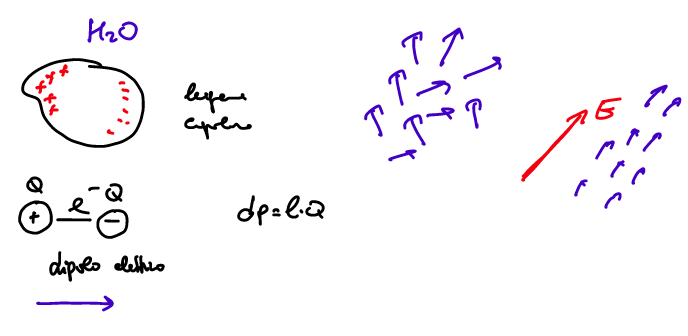
\includegraphics[scale=0.4]{immagini/pol_dip.png}
	\caption{Polarizzazione delle molecole a seguito dell'applicazione di un campo elettrico}
\end{figure}
\\\\Il mezzo viene quindi polarizzato per effetto del campo esterno.\\\\
\paragraph{Polarizzazione Ionica}
Nel corpo umano c'è tanta acqua, quindi è molto importante. Ci sono nel corpo altri materiali solidi, in cui è più difficile riconoscere la molecola in quanto sono organizzati sotto forma di reticolo, dove ogni nodo ha una composizione ionica e quindi una parte positiva ed una negativa ad esempio NaCl: l'Na si va ad "appiccicare" al Cl negativo.\\Nella singola cella, un pezzo è negativo ed uno è positivo, quando si applica un campo E, l'oggetto non può muoversi poiché vincolato, ma può essere deformato, quindi la poralizzazione ha effetto sulla modifica del reticolo, come riassunto nella figura sottostante
\begin{figure}[!h]
	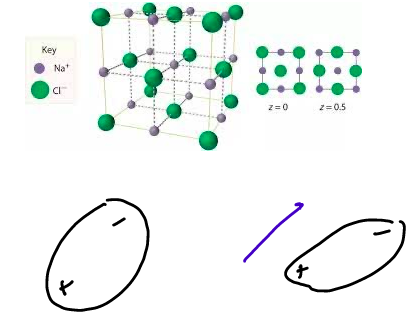
\includegraphics[scale = 0.5]{immagini/pol_io_effetti.png}
	\caption{Effetti della polarizzazione ionica}
\end{figure}
\paragraph{Polarizzazione elettronica}
Questa agisce direttamente sull'atomo, dove abbiamo il kernel positivo e la nube di elettroni. Anche in questo caso, in presenza di un campo E esterno la nube elettronica si può distribuire, su una forma magari più schiacciata, quindi abbiamo ancora un effetto dovuto allo stimolo esterno
\begin{figure}[!h]
	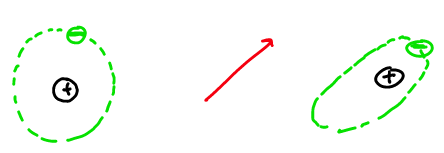
\includegraphics[scale=0.6]{immagini/pol_elettr_effetto.png}
	\caption{Effetti della polarizzazione elettronica}
\end{figure}
\\\\La dissipazione risulta nel momento in cui è necessario trasferire informazione, in quanto occorrono dei segnali sinusoidali, avremo che il campo esterno ha la seguente forma
\begin{figure}[!h]
	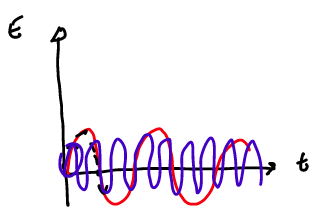
\includegraphics[scale=0.7]{immagini/appl_ce.png}
	\caption{Andamento nel tempo del campo elettrico generato da un segnale sinusoidale}
\end{figure}
\\\\questa applicazione di una forza elettrica alla struttura produce lavoro, siccome la materia vuole stare in un certo modo, la struttura tenderà ad opporsi allo stimolo e quindi ci sarà inerzia che produce attrito e che quindi conseguentemente verrà prodotto un riscaldamento.\\La dissipazione è quindi dovuta alla coesione complessiva dell'organismo che tende a non far muovere le molecole come vogliono.\\È simile a cosa accade con un forno a microonde: se metto del grasso non si cuoce bene, se lo metto in acqua questa cede il calore e lo fa riscaldare più velocemente.\\Se ci fosse una frequenza maggiore, ci sarebbe un ritardo in quanto il corpo umano ha del ritardo per capire che sta succedendo qualcosa e quindi le molecole sono sollecitate contro una forza, ci sarà quindi prima un po' di inerzia per cui ci vuole del tempo prima che la struttura si accorga che sta arrivando un fonte d'onda, ma finché se ne accorge arriva già il fronte negativo e quindi quello che avviene è che l'interazione con la materia è ridotta e concentrata sulla parte esterna.\\\\Occorre ora capire come rappresentare il corpo umano: si usa il modello di Debye, per cui abbiamo
\begin{equation}
	\dot{\epsilon} = \epsilon_{\infty} + \dfrac{\epsilon_s - \epsilon_{\infty}}{1 + j\omega \tau} 
\end{equation}
dove
\begin{itemize}
	\item $\epsilon_s$ è la costante statica (??)
	\item $\epsilon_{\infty}$è la costante ottima
	\item $\tau$ è il tempo di rilassamento, legato al tempo che serve alla molecola per sentire lo stimolo e tornare alla condizione iniziale dopo che lo stimolo è finito. È quindi il ritardo con cui viene seguito lo stimolo
\end{itemize}
Se rappresentiamo consideriamo una rappresentazione grafica:
\begin{figure}[!h]
	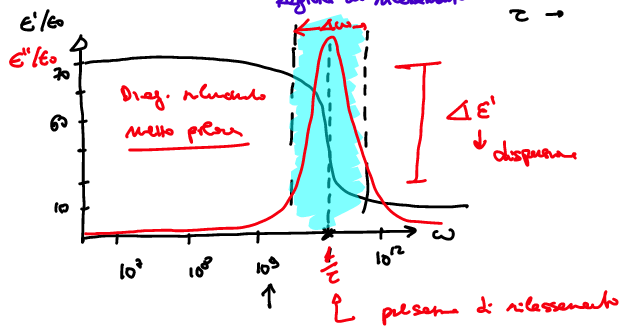
\includegraphics[scale=0.5]{immagini/eps_in_time.png}
	\caption{Andamento del rapporto $\frac{\epsilon'}{\epsilon_0}$ ed $\frac{\epsilon''}{\epsilon_0}$}
\end{figure}
\\\\teniamo conto che i GHz sono nell'ordine $10^9$, mettiamo ad $\frac{1}{\tau}$ la pulsazione di rilassamento.\\Avviene che la parte reale, quindi la capacità di immagazzinare energia e trasmetterla, in prossimità della frequenza in rosso ha un passaggio brusco, in un range di frequenza abbastanza stretto, la regione celeste che è la regione di rilassamento. La parte immaginaria ha un andamento totalmente opposto, in quella finestra c'è un assorbimento importante, le perdite sono elevate e quindi la potenza ceduta viene dissipata dal corpo. Questo è il digramma di rilassamento in un mezzo polare, le conseguenze da un punto di vista di comunicazione è nel che lavorare nella finestra celeste ci sono due fenomeni negativi:
\begin{itemize}
	\item molte perdite, se mando 1W di potenza buona parte del segnale è propagato;
	\item guardando alla permettività, mandando un segnale con una banda importante avrà ogni componente spettrale con una diversa velocità di propagazione e quindi avremo informazione dispersa
\end{itemize}
Quindi tutti i mezzi biologici sono dispersivi, quindi occorre lavorare distanti dalla zona di rilassamento perché il segnale ha effetti dispersivi e distorcenti.\\Visto invece dal punto di vista della fisioterapia, conviene lavorare in quella fascia perché c'è dissipazione e quindi riscaldamento.\\L'acqua ha una pulsazione di rilassamento dell'ordine di 20GHz, quindi il forno a microonde che funziona a 2450 MHz non è molto lontano.\\Questo avverrebbe se ci fossero solo composti polari come l'acqua, ma l'espressione quando consideriamo un corpo umano va adeguata a composti come proteine etc... ottenendo
\begin{equation}
	\dot{\epsilon} = \epsilon' - j \frac{\sigma}{\omega\epsilon_0} = \epsilon_{\infty} + \dfrac{\epsilon_s - \epsilon_{\infty}}{1 + (j \omega \tau)^{1 - \alpha}}
\end{equation}
(dove $0 < \alpha < 1$), 
ottenendo \textbf{l'espressione di Cole-Cole}.\\Mettendo tutto insieme, si è visto che tutto il corpo umano si può rappresentare con 4 di queste espressioni
\begin{equation}
	\dot{\epsilon} = \sum\limits_{i = 1}^{4} \dfrac{\epsilon_{si} - \epsilon_{\infty}}{1 + (j \omega \tau_i)^{1 - \alpha_i}} + \epsilon{\infty} - j \frac{\sigma_0}{\omega}
\end{equation}
dove tutti i parametri con la i e $\sigma$ sono dipendenti dai tessuti del corpo considerato.\\Rappresentando la finestra di dispersione, abbiamo 3 finestre per i vari parametri:
\begin{figure}[!h]
	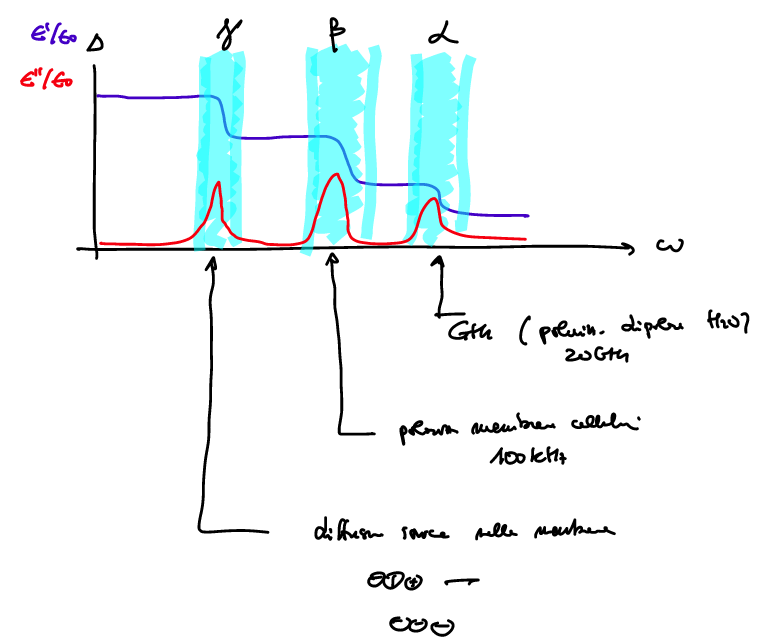
\includegraphics[scale=0.5]{immagini/fin_disp.png}
	\caption{Finestre di dispersione}
\end{figure}
\\\\nelle varie finestre ci sarà un incremento di perdite locale, questa è la risposta del corpo umano tessuto per tessuto (grasso, pelle, ...) in termini di riscaldamento, ed hanno nomi $\gamma$, $\beta$ $\alpha$, dove comandano diversi effetti
\begin{itemize}
	\item[$\gamma$] comanda la polarizzazione dipolare dell'acqua
	\item[$\beta$] comanda la polarizzazione delle membrane cellulari
	\item[$\alpha$] diffusione ionica nelle membrane
\end{itemize}
Immaginando di avere delle cariche libere: applicando il campo questi ioni entrano, poi applicandone un altro escono e quindi c'è assorbimento che produce delle perdite.
\subsection{Come caratterizzare i materiali}
Negli anni 90, sulla spinta dell'evoluzione della telefonia mobile, si è studiato l'impatto del telefono sulla testa e molti gruppi hanno studiato come caratterizzare i tessiti (sugli animali), usando l'espressione come interpolatore ed hanno estratto i parametri che sono di interpolazione. Ci sono dei DB dove in base alla frequenza ed al materiale c'è la lista dei parametri e quindi introducendola nella Cole-Cole generalizzata si ottiene la $\dot\epsilon$.\\Uno dei DB è Italiano, del CNR: niremf.ifac.cnr.it/emfref o /tissprop: si possono scaricare direttamente i parametri oppure avere i valori di permetività e conducibilità: otteniamo diversi valori tra cui la lunghezza d'onda ($\lambda = \frac{\lambda_0}{\sqrt[2]{\epsilon_r}}$). Prendendo ad esempio il muscolo, all'aumentare della frequenza, la conducibilità aumenta, la permettività diminuisce. Più c'è presenza di acqua, più permettività e conducibilità sono elevate.Ne riportiamo alcuni:
\begin{table}
    \begin{tabular}{c|c|c|c|c}
        Tessuto & 10 Mhz ($\frac{\epsilon_r}{\sigma}$) & 434 Mhz & 915 Mhz & 2450 Mhz\\
        \hline
        Grasso & 54 205 & 15 60 & 5 820 & 12 341\\
        Muscolo & 283 715 & 57 1120 & 55 1450 & 50 2272\\
    \end{tabular}
\end{table}
la differenza di conducibilità è importante, quindi il muscolo dissiperà sicuramente più potenza del grasso.
Cerchiamo ora di caratterizzare tutto da un punto di vista ingegneristico
\subsubsection{Assorbimento}
Un'onda arriva su un materiale: una grandezza importante è la densità di potenza dissipata nel corpo
\begin{equation}
	p_j = \frac{1}{2} \sigma \abs{E}^2
\end{equation}
e si misura in $\frac{W}{m^3}$.\\Per le norme di emissione si considera la SAR (Specific Absorption Rate), data da:
\begin{equation}
	SAR = \frac{p_j}{p}
\end{equation}
misurato in $\frac{W}{kg}$ e che indica quanta potenza viene assorbita per unità di massa del dispositivo, ed è quindi data da 
\begin{equation}
	\frac{\partial P}{\partial m} = \frac{1}{2\rho} \sigma \abs{E}^2
\end{equation}
e si usa in quanto è più facile da misurare.\\Se abbiamo un organo e vogliamo calcolare la potenza avremo quindi:
\begin{equation}
	P(\Omega_m) = \int\limits_{\Omega_m} P(r')SAR(r) dr'
\end{equation}
dove 
\begin{equation}
	SAR(\underline{r}) = \frac{1}{2 \rho(r)} \sigma(r) \abs{E(r)}^2 
\end{equation}
Le misure vengono fatte su dei "fantocci" che simulano le caratteristiche EM del corpo, il modo più semplice è usare acqua zucchero e sale:
\begin{itemize}
	\item l'acqua ha una permettività intorno a 70 Ghz
	\item il sale abbassa la $\epsilon_r$
	\item lo zucchero aumenta la $\sigma$
\end{itemize}
Ci sono delle ricette per ricostruire ogni organo e poter quindi misurare il SAR, altrimenti si usano fantocci da "macellaio", pezzi di carne etc...
\subsubsection{Propagazione nei tessuti biologici}
Consideriamo il caso più semplice possibile, dove il corpo umano è un mezzo omogeneo, avrà quindi una permettività $\epsilon' - j \frac{\sigma}{\omega}$.\\Immaginiamo di avere i due mezzi, (1) e (2) e che arrivi un campo elettrico che sia un'onda piana, si propaghi in direzione z, come mostrato in seguito:
\begin{figure}[!h]
	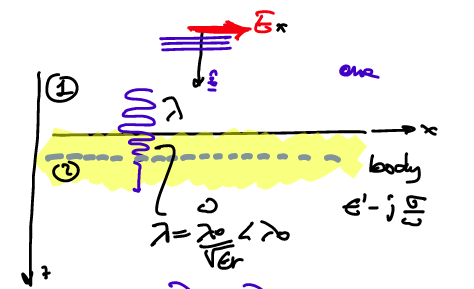
\includegraphics[scale=0.5]{immagini/es_propag.png}
	\caption{Esempio di propagazione di un'onda EM che attraversa due mezzi}
\end{figure}
\\\\Cosa accade al corpo: abbiamo, per un'onda piana
\begin{equation}
	E_x(z) = E_0 e^{-jkz}
\end{equation}
dove k è la costante complessa di propagazione
\begin{equation}
	k = \beta -j \alpha
\end{equation}
ed $\alpha$ e $\beta$ sono rispettivamente il fattore di propagazione ed il fattore di attenuazione:
\begin{equation}
	\alpha = \omega\sqrt[2]{\mu\epsilon'}\{ \frac{1}{2}[ \sqrt[2]{1 + (\frac{\epsilon^{\nu}}{\epsilon'})} -1] \}^{\frac{1}{k}}
\end{equation}
(esponente della quadra forse sbagliata).\\Sia $\alpha$ che $\beta$ dipendono dalla propagazione e dal mezzo.\\L'onda entra nel mezzo e man mano tenderà ad attenuarsi per via delle perdite, è importante capire da che punto in poi possiamo dire che l'onda si sia attenuata: definiamo $\delta_s$ = $\frac{1}{\alpha}$ ed è tale per cui z(profondità)= = $\delta_s$:
\begin{equation}
	\abs{\dfrac{E_x(\delta)}{E_y(\delta)}} = \frac{1}{e}
\end{equation}
che è circa del 37\%, quindi comunicare sotto questa soglia diventa molto complicato, la densità di potenza proporzionale al modulo di E si è ridotta invece del 13\%. Abbiamo un grafico come quello in \ref{sar_att}:
\begin{figure}[!h]
	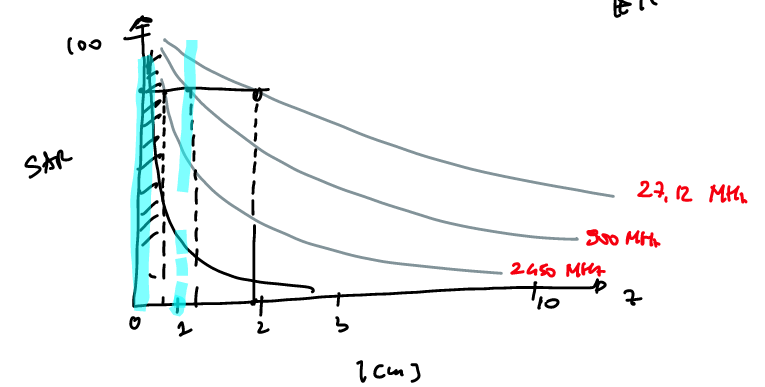
\includegraphics[scale=0.5]{immagini/attenuazione_sar.png}
	\caption{Attenuazione del SAR}
	\label{sar_att}
\end{figure}
\\\\supponiamo di fissare un valore di riferimento del SAR: questo sarà ottenuto nel mezzo, al variare della frequenza, ad una profondità via via crescente: se la profondità diminuisce lo spessore aumenta, quindi aumentando la frequenza otterremmo una profondità di penetrazione molto sottile.\\Fissando la profondità, all'aumentare della frequenza, il SAR tende ad abbassarsi quindi le conseguenze sono che volendo arrivare i profondità per comunicare con un dispositivo in profondità occorre usare frequenze basse, per cui il $\delta_s$ è basso, aumentando la frequenza l'interazione è sempre più in superficie \textbf{\textsf{(ricorda di smentire i coglioni che dicono che il 5G fa male perché entra nel corpo. COJONI, leggete le frequenze usate COJONI)}}.

\chapter{Lezione 3}
\section{Discontinuità fra due mezzi}
Cosa accade quando c'è una discontinutià: il corpo umano può essere rappresenato in modo semplice come un mezzo non omogeneo, quando l'onda incide il corpo umano sperimenterà una serie di effetti. Cosa accade quindi quando l'onda attraversa una superficie: consideriamo una superficie che separi due materiali differenti, materiale 1 e 2: (copia disegnino dagli appunti), immaginiamo di avere determinati campi elettrici e di D(bar). Cosa succede alla potenza rilasciata sul corpo: la distribuzione della potenza dipende dall'incidenza dell'onda, possiamo avere campi elettrici paralleli o normali: dipendentemente dal fatto che il campo arrivi normale o parallelo avremo il \textbf{teorema di continuità dei campi}: a ridosso della discontinuità la componente tangente dei campi si conserva: il campo parallelo sulla discontinuità $\pi$ si conserva senza avere salti, mentre la E normale non si conserva, c'è un salto ma sappiamo che si conserva la componente normale D.\\Da queste considerazioni, cerchiamo di capire le conseguenze sulla distribuzione di potenza a ridosso delle superfici:
1) Polarizzazione tangente: $\underline{E} = \underline{E}||$, avremo che $P = \frac{1}{2}\sigma|E|^2$, avremo le due P, una prima della superficie di separazione ed una dopo: $p_1 = \frac{1}{2}\sigma_1|E_1|^2$ e $p_2 = \frac{1}{2}\sigma_2|E_1|^2$, ne consideriamo il rapporto che sarà dato da $p_1 = \frac{\sigma_1}{\sigma_2}$.\\
2) Pol. normale: riparitiamo da $\frac{p_1}{p_2} = $, dove le componente ortogonali NON sono più uguali come prima, quindi esprimiamo uno in funzione dell'altro: $\epsilon_1E_{ort1} = \epsilon_2E_{ort2}$, ricaviamo $E_{ort1}$ che messo nel rapporto fa si che questo dipenda anche dalla permettività.\\Con degli esempi, CAPIAMO: mezzo 1 è grasso, mezzo 2 è il muscolo. Fissiamo frequenza (dalle libere) f = 434 MHz, abbiamo $\epsilon_r$ e $\sigma$:
\begin{table}
	\begin{tabular}[|c|c|c|]
		& $\epsilon_r$ & $\sigma$\\
		muscolo & 60 & 1\\
		grasso & 15 & 0,1\\
		
	\end{tabular}
\end{table}
nella pol. tangente, avremo che p$_f$ = $\frac{1}{10}$p$_m$ (dove f ed m sono fat e muscle), nella pol. ortogonale avremo $p_f = \frac{16}{10} p_m$, quindi si inverte: in un caso al potenza è maggiore nel muscolo, nell'altro caso nel grasso.\\Come sono gli andamenti:(immagine) la potenza man mano che si scende in profondità si attenua con legge esponenziale. Nel caso tangente, nella discontinuità, la potenza nel grasso è $\frac{1}{10}$ di quella nel muscolo, c'è un salto netto e poi continua a calare per via dell'attenuazione.\\Nel caso parallelo, c'è un salto ma in direzione opposta, perché in questo caso la potenza è maggiore nel grasso.\\L'effetto di assorbimento dei tessuti dipende quindi da come è fatto il dispositivo che genera il campo, in base a come lo genera: se normale, il valore nel muscolo è basso, mentre se parallelo è maggiore e quindi anche l'effetto di esposizione del corpo sarà differente.\\Vediamo ora l'effetto di questa potenza assorbita
\section{Effetti dell'assorbimento di potenza}
L'effetto principale è il riscaldamento ("effetto microonde"), quindi l'esposizione EM ha come effetto principale questo riscaldamento, che in alcuni casi come i sistemi terapeutici è voluto (sempre es. fisioterapia), in molti casi sono effetti collaterali, non voluti quindi si cerca di ridurli. Cerchiamo di capire il legame fra il SAR e la variazione di temperatura nel corpo: c'è l'equazione di Fourier come evolve un processo termico, che nel caso di una sorgente EM ha un pezzo in più: eq per problemi termici:\\$\rho C \frac{dT(t)}{dt} = \Delta (k \Delta T) + p$, dove la temperatura T dipende da tempo e posizione (T(t \underline{r})), $\rho$ è la densità, C è il calore specifico ovvero la quantità di calore assorbita da 1g di sostanza durante la variazione di temperatura di 1° (J/kgC°), k è il coefficiente di conducibilità termica = $\Phi$Q/$\Delta$T (W/m°C), più k è elevato più il mezzo tende ad essere isolante. Infine p è la densità di potenza assorbita (W/m$^3$).\\Ora, è molto più agevole considerare la stessa equazione quando dividiamo ambo i membri per $\rho$, in quanto $\frac{P}{\rho}$ = SAR, questo è il termine "forzante", questa diventa la sorgente del termine noto e quindi rilascia calore e tale potenza è una sorgente che si chiama \textbf{endogena}, in quanto è fornita all'interno del materiale mediante onda EM: se poggiamo un pezzo di metallo caldo su un oggetto, questa è una sorgente esogena, mentre questa si origina dall'interno.\\Nel corpo umano ci sono un paio di peculairità:
- è vivo, quindi si oppone a degli stress esterni, in questo caso il riscaldamento dell'onda EM col sangue che è un sistema di raffreddamento: il vaso si dilata ed il passaggio di sangue toglie calore. C'è un termine che si oppone al riscaldamento
- termine dovuto alla combustione chimica del cibo, che genera energia e si oppone \\\\Otteniamo quindi la nuova equazione, Bioheat equation (Pennes 1948): $\rho C \frac{dT(t)}{dt} = \Delta (k \Delta T) + p + M -B$
dove: M è il metabolismo (W/m$^3$), calore metabolico, la B è la perfusione sanguigna, che ha segno meno perché tende ad opporsi per l'incremento dovuto agli altri termini. B = W(kg/m sigma) c$_b$ (T - T$_{arteria}$), dove T arteria se stiamo bene è di 37°, se questa diminuisce è il sangue che tende a scaldare, altrimenti raffredda. Ma dpo un po' c'è shock termico e quindi il tessuto comincia a bruciare: se ne vediamo l'andamento (schemino)
c'è un punto in cui va giù, ovvero quando la temperatura supera il 44° la perfusione sanguigna non ce la fa più perché il vaso non si più più estendere ed i tessuti necrotizzano.\\Occorre quindi evitare che la temperatura inserita nel corpo dal dispositivo sia vicina ai 43°-44°, altrimenti si arriva a bruciare.\\Ci interessa l'equazione perché c'è un modo semplice per misurare il SAR: il cellulare rilascia un certo SAR nella testa, si parte dall'equazione di Pennes: il termine è istantaneo (primo), poi c'è il termine di conduzione, la M quando c'è una sorgente esterna è piccolo rispetto al calore esterno ed anche la B è un fenomeno lento: il $\tau$ del fenomeno EM è veloce (ordine dei ns), se tocchiamo qualcosa di caldo non è istantaneo capire che si passa ad una temperatura fredda (ordine s), quindi applicando un fenomeno EM in un $\Delta t$ minore di un minuto nell'equaizone rimane solo che $\rho C \frac{dT}{dt} = p$ (circa uguale), quindi dividiamo per $\rho$ ed otteniamo il SAR, che è porporzionale alla variazione di temperatura in un tempo abbastanza breve, quindi la posso approssimare come $C\frac{\Delta T}{\Delta t} \leq$ 1m. Se mettiamo in una bacinella un liquido body-like (acqua zucchero sale) ed introduciamo un telefono cellulare, se facciamo una "foto" all'esterno (con termocamera o sondine), la zona sarà calda verso l'esterno e man mano sempre più fredda, così so può misurare il SAR prodotto dai dispositivi radianti.
\section{Normative EM}
Il progetto del dispositivo deve essere safety by design, quindi devo progettare prima il dispositivo che abbia fra i requisti una certa intensità di campo EM.\\Le attività del capire le soglie di esposizione nasce negli anni 80-90, l'impulso è stato dato dall'esplosione dei telefoni cellulari, c'è stato uno sforzo grande nel 97'-98' per capire quali parametri considerare e come caratterizzarli.\\Prima sono stati fatti degli studi con animali e tessuti espiantati e poi fatta una grossa analisi della letteratura scientifica. Sono stati poi fatti degli studi per cercare di correlare con le malattie (come tumori etc...), si è poi cercato di ridurre gli effetti accertati a breve termine, infine noti gli effetti gli studi si sono spostati sull'individuare le dosi soglia per evitare tali effetti.\\Ci sono due classi di effetti dell'esposizione ai campi EM:
- effetti diretti:\\
- accoppiamento con campi E a bassa frequenza
- accoppiamento con campi B a bassa frequenza
- assorbimento di energia EM.\\Queste 3 tipologie di fenomeno producono due effetti percepibili:\\
- riscaldamento di organi e tessuti, ed è quella più facilmente quantificabile perché produce calore
- stimolazione di nervi e muscoli: c'è un disturbo dovuto al segnale, è possibile che il muscolo si contragga o che vengano stimolati degli effetti chimici e sono difficili da caratterizzare perché sono a lungo termine e sono più difficili da mettere in evidenza.
- effetti indiretti: legati pricipalmente \\
- alle correnti di contatto
- accoppiamento del campo EM con dispositivi impiantati, interazione con un dispositivo impiantato nel corpo. I primi pacemaker erano sensibili al telefono cellulare, sono stati poi protetti con dei filtri.\\\\Sull'analisi e la ricondizione degli effetti sono stati individuati dei limiti: inizialmente sono stati individuati i limiti di base, ovvero wuelli legati alle grandezze EM che producono direttamente l'effetto, ovvero campo E nel corpo, al SAR ed in alcuni casi alla densità di potenza ovvero a grandezze direttamente generate nel corpo e che direttamente correlabili agli effetti diretti.\\Chiaramente cambiano in base alla frequenza, aumentandola, diminuisce la permettività sulla pelle.\\Misurarle è difficile, quindi sono stati introdotti degli insiemi di livelli di riferimento o derivati: sono delle grandezze che si possono valutare in assenza del corpo umano: se abbiamo un cellulare a contatto con la testa, leviamo la testa e calcoliamo le grandezze in un volume che sarebbe stato occupato dalla testa.\\Scelti bene, rispettando i livelli di riferimento allora implicheranno che tali valori verranno rispettati anche quando sarà presente il corpo umano, MA NON vale il viceversa: se vengono rispetta in requisiti di base, non è detto che vengano rispettati quelli di riferimento.\\Le restrizioni di base sono quindi legate alla misurazione "in situ", mentre invece le restrizioni derivate sono misurate in assenza del corpo umano e quindi il loro rispetto implica i primi.\\Abbiamo ad esempio quelli per l'ELF fra 1-100 Khz (metti immagine), poi la microonde (100 Mhz in su), la sperimentazione animale indica come soglia di danno alla salute un incremento della temperatura di 1°C, per legarlo alla grandezza EM si è visto dalle misure che applicando un SAR per 6 min di 4 W/kg si innalza la temperatura di 1°C.\\I limiti di base del SAR sono diversi fra operatori e popolazione: un operatore può essere più esposto in quanto può prendere le dovute precauzioni, (metti tabella) difatti per i lavoratori mediati su 6 min i valori sono circa 5 volte tanto, inoltre la media va fatta sui 10g: se ad un certo punto c'è un hotspot,  possibile superare il limite ma per un punto non posso buttare il dispositivo e quindi si fa una media su 10 g di materiale: si misurano i valori di SAR sui 10g e si fa questa media mobile così da buttare gli outlayers.\\Nel caso di dispositivi wearable, i limiti dei lavoratori sono coincidenti con quelli della popolazione\\Altro aspetto: le analisi vengono spesso fatte nel caso peggiore, ovvero quando sto trasmettebdo una sinusoide, ovvero segnale continuo. Nella realtàm, ogni dispotivo di telemetria ha un \textbf{duty cycle:} ci  sono parti alte e poi periodi di nulla. (metti schemino). In questo, il SAR è pari a DxSAR(continuo): immaginiamo di avere un esempio in cui (vedi esempio): averemo un minuto al giorno in cui il SAR è sopra soglia, ma facendo la media otteniamo $\frac{1}{6}$ del SAR e quindi sotto la soglia di omologazione.\\\\Se però un soggetto è portatore di oggetti come pacemaker i limiti vanno impostati per ogni istante di tempo: se l'attacco è fisico e si produce una potenza molto elevata, questo viene messo fuori uso.\\\\In Italia ed in Europa: il quadro italiano si pone in maniera molto restrittiva rispetto a quelle europee, dove in Europa sono indicati 40 V/m, in Italia ce ne sono 6. Inoltre, ovunque vanno rispettati certi valori, in siti come scuole etc.. ci devono essere valori ancora più bassi, inoltre a regime vanno rispettati dei valori ancora più bassi. La legislazione italiana fissa 3 livelli:
- limite di esposizione: 20 V/m, non devono poter essere misurati in zone che non sono ad esempio dei tralicci recintati
- valore di attenzione: in alcuni ambienti dove ci si viva per un tempo maggiore di 4h consecutive non ci devono essere più di 6 V/m
- obiettivi di qualità: fare in modo che progressivamente in qualunque punto si vada verso i 6 V/m.\\
\subsection{Come fare una valutazione}
Ci si muove su tre livelli a complessità crescente:
1) Misura del campo EM in assenza del corpo umano, andando a misurare i livelli di campo nel volume occupabile dall'uomo, si media per 6 min e si confrontano con i livelli derivati. Se rientrano nella normativa, possiamo omologare il dispositivo
2) Se 1 da valori più elevati, occorre salire di complessità. Qui va fatta una simulazione EM, in cui si introduce il corpo umano, ma può andare bene un fantoccio di forme standard (cubi, cilindi), spesso di materiale omogeneo.\\Con un simulatore si simula il dispositivo e si calcolano campi e SAR nel fantoccio
3) Se ancora i valori sono elevati, si fa una nuova simulazione con un modello antropomorfo, ovvero con tutti i tessuti del corpo umano con la sua permettività e conducibilità  e si valuta il SAR iterando ciascun componente del corpo umano.\\Se non si è conformi, tocca tornare alla progettazione.\\Esistono dei fantocci, il più famoso è visible human (progetto HUGO), un ergastolano che venne messo sotto gelatina, ghiacciato e fatto a fette e dopo la sedia elettrica venne "fotografato". È un fantoccio dove ci sono tutti i tessuti.


\chapter{Lezione 4}
\section{Link bodycentrici - generalità}
Si fa riferimento a quei collegamenti nei quali in qualche modo compare il corpo umano, qui non solo c'è una sorgente che irradia, ma c'è un oggetto che si pone nel mezzo ed è molto complesso (corpo umano).\\Possiamo caratterizzare questi sistemi in base a 
\begin{itemize}
	\item[A)] orientamento della radiazione: immaginiamo di avere un corpo, possiamo avere un'antenna fuori che sta irradiando nel corpo oppure un'irradiazione che dal corpo irradia verso l'esterno.\\Possiamo quindi avere link:
	\begin{itemize}
		\item into the body, dove abbiamo ad esempio:
		\begin{itemize}
			\item sensori
			\item harvester: raccolgono l'energia esterna e la forniscono all'elettronica 
			\item sistemi di telemedicina: possiamo avere un dispositivo che cerca di interrogare dei sensori che sono all'interno del corpo
			\item terapia fisica, ovvero l'irraggiamento del corpo umano ai fini della terapia
		\end{itemize}
		\item out of the body (esterno), dove l'irradiazione dal corpo va verso l'esterno. Abbiamo:
		\begin{itemize}
			\item telemedicina, il sensore trasmette il dato verso l'esterno
			\item sensori
			\item trackers o beacon: dispositivi che servono per identificare la persona. Il dispositivo trasmette informazioni ad esempio sulla posizione
		\end{itemize} 
	\end{itemize}
	\item[B)] tipologia di interazione
	\begin{itemize}
		\item quasi statica, i campi E e B sono poco variabili nel tempo:
		\begin{itemize}
			\item induttivo, si lavora principalmente col campo B
			\item di tipo capacitivo, in cui si lavora col campo E 
		\end{itemize}
		\item zona di midfield, è una zona intermedia che domina molte delle applicazioni body centriche, non siamo più nel campo lontano ma non possiamo più separare campo elettrico e magnetico
		\item radiativa, abbiamo che i campi non sono più così separabili
	\end{itemize}
\end{itemize}
Immaginiamo di avere un elemento radiante, ed una corrente (antenna di cellulare, smartwatch etc...) ed avere r che è la distanza dominante: abbiamo 3 regioni (copia immagine).\\Abbiamo che nella zona di far field il campo elettrico e magnetico sono fra loro ortogonali, (anche a k che è la direzione di propagazione) e la densità di potenza è reale ed è proporzionale al campo elettrico, (copia tutte le formule)\\Nella zona induttiva, che è il near field, il campo varia molto lentamente l'energia è induttiva(??) ma possiamo usarla per far colloquiare due dispositivi, ci sono tutte le componente e sono mischiare e non si possono separare. Poi c'è la zona di mezzo dove comunque non si segue $\frac{1}{r}$.\\Va tenuto chiaro che: nelle zone vicine, quando abbiamo a che fare col corpo umano, c'è energia reattiva che  magnetostatica o elettrostatica che NON si propaga ma si può "raccogliere" ed accoppiare e quindi usare per le applicazioni.\\\\Un altro aspetto importante sono le frequenze di lavoro:
\begin{itemize}
	\item basse, Low Frequency ed High Freqeuncy (kHz - MHz), le LF vanno 30-300 KHz, mentre HF 2-30MHz. Sono tipiche dei sistemi quasi statici, quando lavoriamo con queste stabiliamo un regime quasi statico e quindi tutto interviene in campo quasi statico. Qui il campo si attenua di meno quando interagisce col corpo, lo spessore pelle è maggiore ma sono coinvolti dei dispositivi più grandi. Se volessi con una sola antenna trasmittente leggere tante antenne del corpo umano dovrei usare queste frequenza
	\item elevate, UHF e microwave. Le UHF sono 300 MHz - 3GHz, mentre le microvawe sono da 1 - 3GHz.  Sono tipiche dei sistemi radiativi. Penetrano meno, circa 4cm nel corpo e quindi possono interagire con la pelle meglio (penetrano meno) ma hanno come vantaggio di permettere l'utilizzo di antenne più basse.
	\item 
\end{itemize}
L'antenna è un oggetto poco miniaturizzabile, quindi in molti dispositivi l'ingombro è dovuto alla presenza di antenne (similmente a quanto accade per la batteria) soprattutto se l'antenna deve essere piccola.\\\\Altro aspetto importante sono le geometrie, i layout
\begin{itemize}
	\item in dispositivi quasi statici, abbiamo 
	\begin{itemize}
		\item coil, avvolgimenti nei sistemi magneto-statici
		\item piastre, che svolgono la funzione di condensatore
	\end{itemize}
	\item in sistemi radiativi abbiamo
	\begin{itemize}
		\item dipoli
		\item loop
		\item slot
		\item patch
	\end{itemize}
\end{itemize}
Seguono poi le tipologie di servizio, ovvero perché usiamo il sistema bodycentrico:
\begin{itemize}
	\item comunicazione: uno degli scopi principe.\\Sistemi wearable, con cui è possibile fare delle body area network. Ad esempio, in ambito militare, quando vanno in missione c'è una rete mash fra i vari soldati: ognuno ha una radio che permette di stabilire una comunicazione con gli altri fino ad arrivare al capo
	\end{itemize}
	\item telemetrica e comando: abbiamo un dispositivo sul corpo o al suo interno, che deve mandare un messaggio all'esterno (telemetria). Il comando invece serve principalmente a configurare dei dispositivi impiantati: le pompe ad infusione, dispositivi che rilasciano farmaco, neurostimolatori periodicamente vanno controllate dagli esperti del settore (\textbf{\textsf{NON NOI}}).
	\item Wireless Power Trasnfer: trasferimento di energia per alimentare un dispositivo che non ha batteria o per evitare che la batteria di un dispositivo venga consumata per comunicare.\\Anche se un dispositivo medico non ha la batteria si cerca di non usarla i più possibile, quindi l'energia che serve per comunicare viene fornita dall'esterno.\\L'esempio classico è la ricarica del cellulare o dello spazzolino elettrico
	\item Marker / Labeling: alcuni dispositivi medici possono essere dei \textbf{marcatori}. I marker non trasmettono informazione, ma servono ad esempio per centrare il corpo umano rispetto a qualche altra sorgente.\\Il labeling è l'associazione al dispositivo medico un codice, simile al codice a barre, fatto a radiofrequenza da sistemi RFID quindi si può assegnare un identificavo ad un oggetto per leggere e scrivere dentro. Si fa quindi identificazione e tracking, ma anche localizzazione.
\end{itemize}

\subsection{Architetture di comunicazione}
Abbiamo due modalità per stabilire un link:
\begin{itemize}
	\item link simmetrici
	\item link asimmetrici
\end{itemize}
differiscono sostanzialmente nella gerarchia con cui uno trasmette ed uno riceve, c' è differenza nei protocolli usati, nella progettazione hadrware etc...

\subsubsection{Link simmetrici}
In un link in generale abbiamo due oggetti, A e B che devono scambiarsi delle informazioni.\\In un link simmetrico, possiamo definire trasmettitore TX e ricevitore RX: TX manda il segnale ed RX deposita tale segnale su un carico.\\È possibile anche che si scambino i ruoli fra i due ad un certo punto, quindi non parlano mai contemporaneamente (half duplex). L'esempio classico sono il cellulare che parla con stazione RB e poi altro cellulare, o anche i walkie talkie.\\Ambe due i dispositivi hanno la stessa elettronica e serve una fonte locale di alimentazione, quindi o una alimentazione ad un cavo fisico oppure una batteria.\\Esempi: bluetooth BT, che funziona a 2450 MHz, bluetooth BLE (low energy) che permette di avere una durata della batteria più lunga: la prima cosa da fare è il pairing fra i dispositivi.\\LTE (ex 4G), che è Long Term Evolution, 850-900 - 2100 MHz, ci sono i sistemi UMTS, CDMA, SCDMA\\Wi Fi, le cui frequenze sono 2450 - 5800\\5G, che ha diverse frequenze, 700 MHz, LTE, 3600Mhz, 26GHz fino a 60 GHz.\\Sistemi IoT: LoRa (Long Range) e SIGFOX: sono sistemi di Wireless Lan, sistemi con cui interconnettere oggetti e quindi molto usati in sistemi di IoT, possono collegarsi ad un hotspot tipo WiFi ma con range molto più alto e con batterie che durano molto tempo (ordine anni). Le frequenze sono più basse, 433 Mhz e 868 Mhz.

\subsubsection{Link asimmetrici}
Altra filosofia, che è molto gerarchizzata: tipicamente c'è un oggetto che si chiama lettore (Reader) che va ad interrogare un altro oggetto "stupido" da un punto di vista dell'elettronica e risponde per riflessione, quindi non ha sensori ma in qualche modo riflette il segnale modulandolo (copia disegnino) in modo da poter codificare i valori 0 ed 1. Per farlo, c'è un interruttore del D che permette di modulare ma è molto semplice e non richiede batteria o elettronica complessa, tutta l'energia che serve per attivare l'interruttore arriva dal trasmettitore, a differenza invece del Reader.\\Ci sarà un link diretto dal lettore al trasmettitore e poi un link inverso che va dal dispositivo al reader.\\In questo caso i due dispositivi possono mandare segnali contemporaneamente, quindi con comunicazione full duplex. Abbiamo dispositivi monouso, come cerotti che evitano l'uso di batterie e costano meno.

\subsection{Efficienza dei collegamenti}
Quando si fa un collegamento, una delle cose più preziose è l'energia, in quanto sistemi wearable non possono essere collegati alla corrente e quindi tutta l'energia è data dalla batteria che non ha durata lunga, inoltre nel corpo umano si perde tanta energia per via delle perdite.\\Introduciamo in due step:
\begin{itemize}
	\item[1] solo antenna che trasmette in prossimità del corpo umano, ad esempio l'orologio che prova a collegarsi al wifi: abbiamo il corpo, un dispositivo che sta irradiando e che produce una radiazione che poi entra magari nel corpo.\\Consideriamo poi una superficie che racchiude tutto, potremmo applicare il thm di Pointying, abbiamo della potenza irradiata, della potenza dissipata nel corpo (P$_j$), quindi la potenza totale che fornisco è $P = P_r + P_j(k) + $, se abbiamo un sistema di comunicazione deve prevalere la potenza irradiata, mentre invece per sistemi che fanno terapia deve prevalere quella dissipata.\\\\Possiamo caratterizzare la bontà del trasmettitore in base alla efficienza $\ni_R = \frac{P_R}{P}$ (copia pedici + formule), abbiamo in più il termine (verde) che è proprio specifico della presenza del corpo.Si possono anche associare le resistenze delle antenne.\\Quando non c'è il corpo umano, la $R_R$ tende ad andare proporzionalemnte come il raggio dell'antenna, l'andamento è simile a questo (metti immagine), le prestazioni migliorano ingrandendo l'antenna in modo da avere una resistenza di radiazione migliore ed enfatizzare quindi la parte radiata.\\Se abbiamo anche il corpo, aumentando le dimensioni dell'antenna irradia meglio ma manda più potenza nel corpo e ci sarà maggiore dissipazione. Se $\frac{R}{\lambda}$ aumenta abbiamo due effetti opposti:
	\begin{itemize}
		\item da una parte aumenta la resistenza di radiazione
		\item ma da una parte aumenta anche la resistenza di perdita
	\end{itemize}
	(copia ASSOLUTAMENTE L'IMMAGINE DEL DONDOLO)-\\Nei sistemi radianti, non comanda la lunghezza in se, ma la lunghezza RISPETTO alla lunghezza d'onda. Abbiamo il seguente andamento:\\ ad un certo punto, superato questo, il dispositivo irradierebbe come uno piccolo e quindi sarebbe poco efficiente.\\È un tradeoff e vale ogni volta che abbiamo un mezzo con perdite (pelle, pneumatico, etc...) l'effetto di portare un dispositivo in prossimità di un mezzo avrà un valore ottimale e tale valore ottimale dipende poco dalla forma dell'antenna (dipolo, loop, slot) ma tanto dalla forma: gli oggetti fatti a loop hanno una l$_{max}$ ottimale in termini di ingombro.
	\item[2] Consideriamo ora anche il link in presenza del corpo umano.\\Possiamo avere la seguente immagine:\\un'antenna che irradia, chiamiamo P$_l$ la potenza che verrà raccolta per far funzionare il dispositivo. Il parametro che descrive quanto p efficiente questo trasferimento di potenza dal tx all'oggetto è il PTE: $\frac{P_L}{P_{in}}$ e va massimizzato per avere un link efficiente.\\Dipenderà anche in questo caso dai tessuti, dalla posizione rispetto al corpo (più in profondità, maggiore l'attenuazione), dipende anche dalla forma delle antenne coinvolte ed ovviamente dalla frequenza (PTE tende a diminuire quando la frequenza aumenta perché l'attenuazione del corpo aumenta ed è quindi più difficile eseguire il comportamento).\\Possiamo scrivere $P_L = P_{in} \cdot PTE$, fissando la PTE, per aumentare la P$_L$ va aumentata la $P_{in}$, ma nel corpo aumenta anche il SAR ovvero la potenza rilasciata: qui il problema è che per aumentare la P$_L$ potremmo aumentare la potenza in ingresso ma se aumenta troppo il SAR sforo i limiti di legge e qui si capisce bene cosa vuol dire safety by design.\\Il primo anello della catena di progettazione deve:
	\begin{itemize}
		\item SAR $< SAR_{max}$
		\item P$_{in}$ < P max
	\end{itemize} 
	viene quindi fuori un vincolo per la PTE, imposto dal SAR: questo ci dice quindi quanto deve essere fatto bene il collegamento in modo da poter minimizzare la potenza necessaria.
\end{itemize}

\section{Link in near field}
Negli anni di fine 800 (1831) vengono fatti i primi studi da Faraday sulla induzione EM: gli studi avevano a che fare con due coil, in modo che questi potessero trasferirsi energia senza che questi si toccassero. L'accoppiamento veniva fatto mediante l'uso di materiale ferromagnetico, per molti anni venne usato ad esempio nei trasformatori ma non per la comunicazione.\\Agli inizi del 1900 ci sono gli esperimenti di Hertz e di Tesla, dove si parla proprio di trasmissione di informazione a distanza, Telsa introdusse anche i concetti di risonanza in quanto la sua ambizione era rifornire l'energia nelle città tramite una torre che mandava energia sulle case della città.\\Sono applicate nelle comunicazioni a bassa frequenza e piccola distanza, in ambito medico abbiamo dispositivi IMD (Implanted Medical Device) che possono essere pacemaker, defibrillatori, neurostimolatori etc... la comunicazione viene stabilita con un altro coil messo sulla superficie del body stabilendo un link a bassa frequenza. Sono link di tipo quasi statico, basati o su accoppiamento induttivo, o su accoppiamento induttivo risonante o accoppiamento capacitivo. Le frequenze di lavoro sono le HF ed LF, anche attorno ai KHz: in queste condizioni la capacità di conduzione del corpo è bassa, quindi basse perdite che permettono di avere PTE elevata, inoltre la permettività è elevata.\\I dispositivi non sono vere e proprie antenne, sono una specie di elettrodi in quanto lavorano in campo vicino.




\part{Parte Localization}








\part{Parte Hardware}









































\end{document}
